% Biên dịch bằng XeLaTeX (Overleaf: Menu > Compiler > XeLaTeX). Phông TeX Gyre Termes / Cursor có sẵn trong TeX Live.
\documentclass[12pt,a4paper]{article}
\usepackage[top=2.5cm,bottom=2.5cm,left=3cm,right=2.5cm]{geometry}
\usepackage{fontspec}
\setmainfont{TeX Gyre Termes}
\setsansfont{TeX Gyre Heros}
\setmonofont{TeX Gyre Cursor}[Scale=0.9]
\usepackage{polyglossia}
\setmainlanguage{vietnamese}
\usepackage{graphicx,booktabs,tabularx,array,multirow,float,caption,enumitem,xcolor,amsmath}
\usepackage{tikz}
\usetikzlibrary{positioning,arrows.meta,shapes.geometric,fit,calc}
\usepackage[colorlinks=true,linkcolor=blue!50!black,urlcolor=blue!50!black,citecolor=blue!50!black]{hyperref}
\captionsetup{font=small,labelfont=bf}
\setlength{\parskip}{4pt}\setlength{\parindent}{0pt}
\renewcommand{\arraystretch}{1.12}
\newcommand{\TODO}[1]{\textcolor{red}{\textbf{[CẦN ĐIỀN: #1]}}}
\newcommand{\ci}[2]{{\scriptsize[#1, #2]}}
\newcolumntype{Y}{>{\raggedright\arraybackslash}X}
\newcolumntype{R}{>{\raggedleft\arraybackslash}X}

\begin{document}

%================ BÌA ================
\begin{titlepage}
\centering\vspace*{1.5cm}
{\large Môn học DPL302m}\\[0.4cm]
{\Large\bfseries Nhận dạng tiếng nói tiếng Việt kèm dịch sang tiếng Anh}\\[0.3cm]
{\large Vietnamese Speech Recognition with English Translation}\\[1.2cm]
{\Large\bfseries BÁO CÁO TIẾN ĐỘ TASK 2}\\[0.3cm]
{\large Xử lý dữ liệu, thực nghiệm Baseline và phát triển Proposed Method}\\[1.8cm]
{\large\bfseries Nhóm 5}\\[0.6cm]
\begin{tabular}{l}
Phạm Nguyễn Khánh Nguyên (SE200641)\\
Trần Thanh Vũ (SE200433)\\
Hà Lê Thành Nhân (SE201028)\\
\end{tabular}\\[2cm]
\end{titlepage}

\tableofcontents
\newpage

%================ TÓM TẮT ================
\section*{Tóm tắt}
\addcontentsline{toc}{section}{Tóm tắt}
Đề tài xây dựng và so sánh ba hệ thống chuyển giọng nói tiếng Việt thành văn bản tiếng Anh: \textbf{A} (PhoWhisper-small nhận dạng, rồi OPUS-MT vi--en gốc dịch), \textbf{B} (cùng ASR, OPUS-MT được fine-tune trên giả thuyết ASR của PhoWhisper ghép với bản dịch giả của VinAI Translate v2) và \textbf{C} (SeamlessM4T-v2-large dịch trực tiếp từ audio, không huấn luyện thêm). Nhóm dùng A và C làm hai baseline; B là Proposed Method V1.

Dữ liệu huấn luyện là 55\,000 mẫu lấy ngẫu nhiên (seed 42) từ VietSpeech (61,2 giờ; chia 49\,500 train / 5\,500 dev). Đánh giá trên toàn bộ FLEURS tiếng Việt (4\,212 bản ghi, 1\,978 câu, 13,3 giờ), điểm chính tính trên các bản ghi $\le$ 30 giây (4\,199 bản ghi) với khoảng tin cậy 95\% bootstrap theo câu duy nhất.

Kết quả chính (SacreBLEU): A đạt 16,33; B đạt 17,24 (+0,91, KTC 95\% [0,50; 1,35] so với A); C đạt 27,75 (+11,42 so với A). Fine-tune trên giả thuyết ASR chỉ cải thiện nhỏ so với A và \emph{chưa} cho thấy ưu thế so với fine-tune trên transcript sạch (+0,14, KTC [$-$0,14; 0,40]). Phân tích lỗi chỉ ra bốn nguồn lỗi chính: số đọc thành chữ, tên riêng và từ mượn bị ASR phiên âm sai, dịch lặp vòng, và khoảng cách miền dữ liệu giữa VietSpeech (câu ngắn, trung bình 4,0 giây) với FLEURS (11,3 giây). Phiên bản V2 (chặn lặp khi giải mã) loại gần hết lỗi lặp nhưng chỉ tăng +0,14 BLEU.

%================ TỔNG QUAN ================
\section{Bài toán và thiết kế hệ thống}
\subsection{Ba hệ thống}
\begin{figure}[H]\centering
\begin{tikzpicture}[node distance=7mm, every node/.style={font=\small}, box/.style={draw,rounded corners=2pt,minimum height=8mm,align=center,fill=blue!6}, arr/.style={-{Stealth[length=2mm]}}]
\node[box,fill=gray!15] (aud) {Audio\\tiếng Việt};
\node[box,right=of aud] (asr) {PhoWhisper-small\\(ASR, beam 3)};
\node[box,right=of asr,yshift=7mm] (mta) {OPUS-MT gốc\\\textbf{(A)}};
\node[box,right=of asr,yshift=-7mm,fill=orange!15] (mtb) {OPUS-MT fine-tune\\\textbf{(B)}};
\node[box,right=of mta,fill=gray!15] (outa) {Văn bản\\tiếng Anh};
\node[box,below=12mm of mtb,xshift=6mm,fill=green!10] (seam) {SeamlessM4T-v2-large, S2TT (beam 4)\\\textbf{(C)}};
\node[box,right=of mtb,fill=gray!15] (outb) {Văn bản\\tiếng Anh};
\draw[arr] (aud)--(asr); \draw[arr] (asr)--(mta); \draw[arr] (asr)--(mtb); \draw[arr] (mta)--(outa); \draw[arr] (mtb)--(outb);
\draw[arr] (aud) |- (seam); \draw[arr] (seam) -| (outb);
\end{tikzpicture}
\caption{Ba hệ thống: A và B dùng chung đầu ra ASR và khác nhau ở mô hình dịch; C đi thẳng từ audio sang văn bản tiếng Anh.}
\end{figure}
\begin{itemize}[nosep]
\item \textbf{A (baseline 1):} PhoWhisper-small~\cite{phowhisper} $\rightarrow$ OPUS-MT vi--en~\cite{opusmt}, cả hai dùng nguyên bản, không huấn luyện thêm.
\item \textbf{B (Proposed V1):} cùng ASR; OPUS-MT được fine-tune trên cặp (giả thuyết ASR tiếng Việt, bản dịch tiếng Anh) để mô hình quen với lỗi ASR.
\item \textbf{C (baseline 2):} SeamlessM4T-v2-large~\cite{seamless}, dịch giọng nói sang văn bản (S2TT) zero-shot.
\end{itemize}
\subsection{Giao thức đánh giá}
Toàn bộ FLEURS tiếng Việt (train, validation, test) được dùng làm tập kiểm tra, vì tập test riêng chỉ có 857 bản ghi / 347 câu. Hệ thống không được huấn luyện trên FLEURS. Nhóm báo cáo: WER và CER cho ASR; SacreBLEU (mặc định, phân biệt hoa thường) và chrF++ cho dịch; khoảng tin cậy 95\% bằng bootstrap 1\,000 lần lấy mẫu lại \emph{theo câu duy nhất} (các bản ghi cùng một câu được lấy mẫu cùng nhau), độ chênh giữa hai hệ thống dùng bootstrap cặp. Điểm \emph{chính} tính trên bản ghi $\le$ 30 giây (4\,199 bản ghi, 1\,974 câu); điểm \emph{phụ} tính trên tất cả. Cả ba hệ thống chỉ nghe tối đa 30 giây đầu của mỗi bản ghi.

%================ CHƯƠNG I ================
\section{Xử lý và phân tích dữ liệu}
\subsection{Thống kê nguồn dữ liệu}\label{sec:source}
\begin{table}[H]\centering\small
\begin{tabularx}{\textwidth}{>{\raggedright\arraybackslash}p{2.2cm}p{1.4cm}Y>{\raggedleft\arraybackslash}p{2.6cm}p{1.3cm}}
\toprule
Nguồn & Loại & URL / cách thu thập & Số lượng mẫu & Định dạng \\\midrule
VietSpeech (MMLab-UIT) & Online & \url{https://huggingface.co/datasets/NhutP/VietSpeech}; giọng nói từ nhiều nguồn mạng xã hội, đủ giọng Bắc, Trung, Nam; giấy phép Apache-2.0 &
bộ gốc 1\,026\,047 mẫu (hơn 1\,100 giờ, 131 GB); nhóm dùng 55\,000 mẫu (61,2 giờ) & wav, 16 kHz \\
FLEURS tiếng Việt & Online & Google FLEURS (\url{https://arxiv.org/abs/2205.12446}); câu đọc có bản dịch tiếng Anh (FLORES) & 4\,212 bản ghi, 1\,978 câu, 13,3 giờ; 3,06 GB (2,85 GiB) & wav \\
\bottomrule\end{tabularx}
\caption{Nguồn dữ liệu. Nhóm không thu thập dữ liệu offline.}
\end{table}
\textbf{Các trường dữ liệu.} VietSpeech (metadata của nhóm): \texttt{id, source\_index, audio\_path, vi\_text, sampling\_rate, audio\_format, en\_text}. FLEURS (metadata của nhóm): \texttt{split, fleurs\_id, audio\_path, vi\_script, en\_script, flores\_id, flores\_split, match\_status, sampling\_rate, duration\_sec}. Cột \texttt{sampling\_rate} trong cả hai metadata bị trống; tần số lấy mẫu của VietSpeech là 16 kHz theo thẻ dữ liệu của bộ gốc. Nhóm dùng 100\,000 mẫu đầu của bộ gốc, từ đó lấy ngẫu nhiên 55\,000 mẫu (seed 42); cỡ 55\,000 được chọn sau khi đo tài nguyên trên Colab (Tesla T4) để vừa ngân sách GPU.

\textbf{Nhãn tiếng Anh của VietSpeech là nhãn giả.} Bộ gốc chỉ có transcript tiếng Việt. Cột \texttt{en\_text} do nhóm tạo bằng mô hình VinAI Translate v2 (vi$\rightarrow$en, beam 4) dịch từ \texttt{vi\_text}. Chất lượng của các bản dịch này chưa được đánh giá bởi người, nên điểm các mô hình fine-tune bị chặn bởi chất lượng nhãn giả.

\subsection{Phương pháp làm sạch và gán nhãn}
\begin{figure}[H]\centering
\begin{tikzpicture}[node distance=6mm, every node/.style={font=\scriptsize}, box/.style={draw,rounded corners=2pt,minimum height=9mm,text width=2.7cm,align=center,fill=blue!6}, arr/.style={-{Stealth[length=2mm]}}]
\node[box] (v1) {VietSpeech\\(100\,000 mẫu đầu)};
\node[box,right=of v1] (v2) {Kiểm tra \texttt{id} duy nhất, bỏ dòng rỗng};
\node[box,right=of v2] (v3) {Hoán vị seed 42, lấy 55\,000 mẫu};
\node[box,below=8mm of v3] (v4) {Chia dev 5\,500 / train 49\,500};
\node[box,left=of v4] (v5) {ASR PhoWhisper (beam 3): 0 lỗi, 0 rỗng};
\node[box,left=of v5,fill=orange!15] (v6) {Sửa \texttt{n't} ở nhãn Anh (4\,095 câu)};
\node[box,below=8mm of v6,fill=orange!15] (v7) {Dữ liệu fine-tune: (giả thuyết ASR, nhãn Anh)};
\draw[arr](v1)--(v2);\draw[arr](v2)--(v3);\draw[arr](v3)--(v4);\draw[arr](v4)--(v5);\draw[arr](v5)--(v6);\draw[arr](v6)--(v7);
\end{tikzpicture}\\[4mm]
\begin{tikzpicture}[node distance=6mm, every node/.style={font=\scriptsize}, box/.style={draw,rounded corners=2pt,minimum height=9mm,text width=2.7cm,align=center,fill=green!10}, arr/.style={-{Stealth[length=2mm]}}]
\node[box] (f1) {FLEURS\\4\,212 bản ghi};
\node[box,right=of f1] (f2) {\texttt{match\_status} = matched (4\,212)};
\node[box,right=of f2] (f3) {Ghép đường dẫn, mono 16 kHz, cắt 30 s};
\node[box,right=of f3] (f4) {Đánh giá A, B, C};
\draw[arr](f1)--(f2);\draw[arr](f2)--(f3);\draw[arr](f3)--(f4);
\end{tikzpicture}
\caption{Quy trình xử lý dữ liệu VietSpeech (trên) và FLEURS (dưới).}\label{fig:flow}
\end{figure}
\begin{itemize}[nosep]
\item \textbf{Trùng lặp.} VietSpeech: kiểm tra \texttt{id} duy nhất; \emph{chưa} kiểm tra trùng nội dung văn bản hay âm thanh (hạn chế, xem mục~\ref{sec:limit}). FLEURS: không loại bản ghi trùng câu, vì mỗi câu có nhiều giọng đọc khác nhau (trung bình 2,13 bản ghi/câu); thay vào đó bootstrap lấy mẫu theo câu. Số câu trùng giữa các tập (train--test, train--validation, validation--test) là 0.
\item \textbf{Giá trị thiếu.} Loại dòng có \texttt{vi\_text} hoặc \texttt{en\_text} rỗng, và dòng ASR lỗi hoặc rỗng. Ở bước huấn luyện MT số dòng bị loại là 0 trên 55\,000 mẫu. FLEURS: cả 4\,212 dòng đều \texttt{matched}.
\item \textbf{Nhiễu.} Không lọc nhiễu âm thanh; giữ nguyên để phản ánh dữ liệu mạng xã hội. Bản ghi FLEURS dài hơn 30 giây (13 bản ghi) bị cắt còn 30 giây và được tách khỏi điểm chính.
\item \textbf{Chuẩn hóa.} Âm thanh: mono, 16 kHz (tự đổi tần số khi file khác 16 kHz). Văn bản tiếng Việt cho WER: Unicode NFC, chữ thường, bỏ dấu câu. Nhãn tiếng Anh: sửa lỗi tách \texttt{n't} của bản dịch VinAI (ví dụ ``do n't'' $\rightarrow$ ``don't'') bằng biểu thức chính quy; ảnh hưởng 4\,095/55\,000 câu (7,4\%).
\item \textbf{Gán nhãn.} Không có gán nhãn thủ công: transcript tiếng Việt lấy từ bộ dữ liệu gốc, bản dịch tiếng Anh là nhãn giả (mục~\ref{sec:source}). Vì vậy \textbf{không áp dụng} độ đồng nhất giữa người gán nhãn (Cohen/Fleiss Kappa). Công cụ gán nhãn: không dùng.
\end{itemize}

\subsection{Thống kê mô tả và phân bố}\label{sec:stats}
\textbf{Bài toán không có lớp.} Dữ liệu nhận dạng và dịch tiếng nói không có nhãn phân lớp, nên ``mất cân bằng lớp'' không áp dụng. Nhóm thay bằng phân tích phân bố độ dài, số từ và số bản ghi trên câu, và \emph{khoảng cách phân bố} giữa dữ liệu huấn luyện và dữ liệu đánh giá.

\begin{table}[H]\centering\small
\begin{tabular}{lrrrrr}\toprule
Tập & Mẫu / bản ghi & Câu duy nhất & Giờ & Số từ vi (TB) & Số từ en (TB)\\\midrule
VietSpeech dev & 5\,500 & -- & 6,18 & 14,37 & 11,13\\
VietSpeech train & 49\,500 & -- & 55,01 & 14,28 & 11,03\\
\textbf{VietSpeech (tổng)} & \textbf{55\,000} & -- & \textbf{61,19} & 14,29 & 11,04\\\midrule
FLEURS test & 857 & 347 & 3,00 & \multicolumn{2}{c}{}\\
FLEURS validation & 361 & 149 & 1,19 & \multicolumn{2}{c}{}\\
FLEURS train & 2\,994 & 1\,482 & 9,08 & \multicolumn{2}{c}{}\\
\textbf{FLEURS (tổng)} & \textbf{4\,212} & \textbf{1\,978} & \textbf{13,27} & 29,12 & 20,92\\
\bottomrule\end{tabular}
\caption{Chia tập. VietSpeech chia 90/10 (train/dev) theo hoán vị seed 42; FLEURS không dùng để huấn luyện, dùng toàn bộ để đánh giá. Số từ trung bình của dev và train VietSpeech gần như bằng nhau (14,37 và 14,28).}\label{tab:splits}
\end{table}

\begin{table}[H]\centering\small
\begin{tabular}{lrrrrrrr}\toprule
 & min & p25 & trung vị & p75 & p95 & max & TB\\\midrule
\multicolumn{8}{l}{\emph{Thời lượng (giây)}}\\
VietSpeech (55\,000) & 2,0 & 2,7 & 3,6 & 5,0 & 7,2 & 8,0 & 4,0\\
FLEURS (4\,212) & 2,5 & 8,5 & 10,7 & 13,3 & 18,7 & 42,2 & 11,3\\\midrule
\multicolumn{8}{l}{\emph{Số từ tiếng Việt}}\\
VietSpeech & 3 & 10 & 13 & 18 & 27 & 44 & 14,3\\
FLEURS & 7 & 22 & 28 & 35 & 48 & 75 & 29,1\\\midrule
\multicolumn{8}{l}{\emph{Số bản ghi trên mỗi câu (FLEURS)}}\\
 & 1 & 2 & 2 & 3 & 3 & 3 & 2,13\\
\bottomrule\end{tabular}
\caption{Thống kê mô tả. VietSpeech không có mẫu nào dài hơn 8 giây; FLEURS có 13 bản ghi (0,31\%) dài hơn 30 giây.}\label{tab:desc}
\end{table}
\begin{figure}[H]\centering
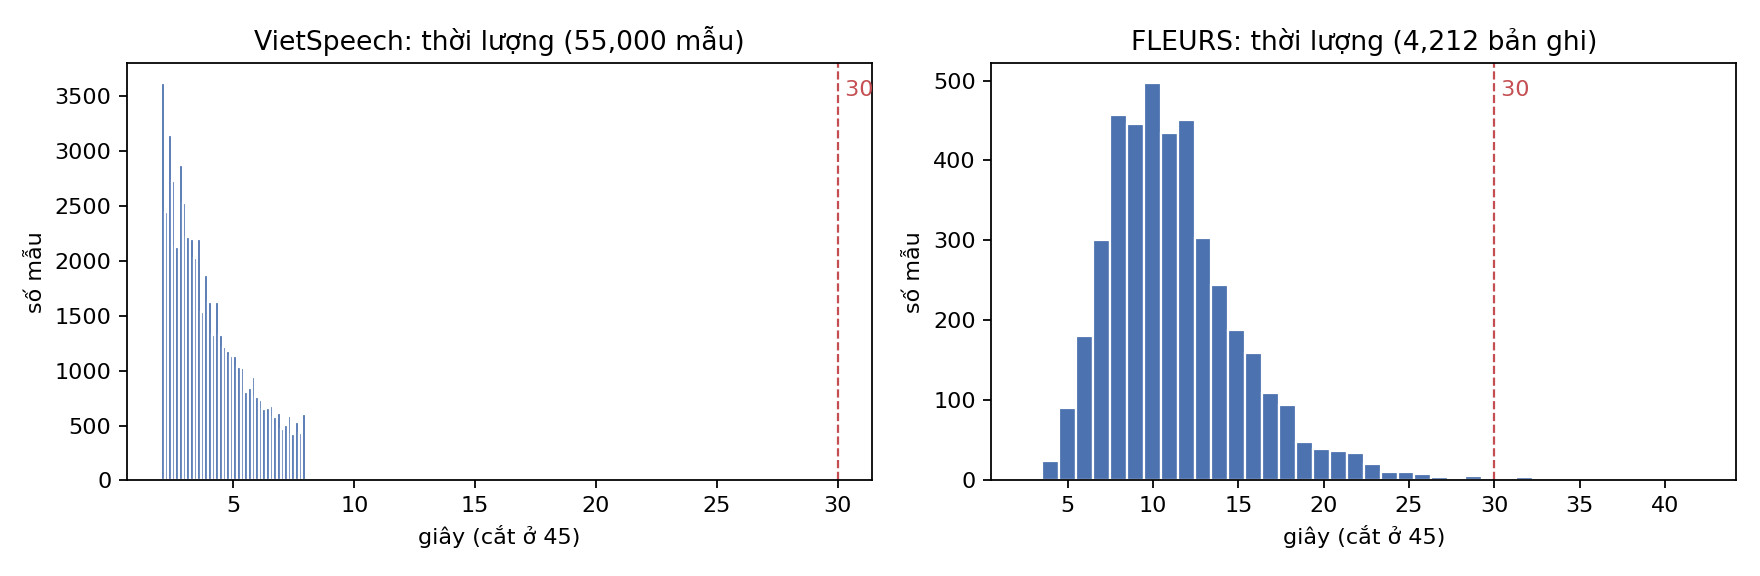
\includegraphics[width=.95\textwidth]{figs/duration_hist.png}\\
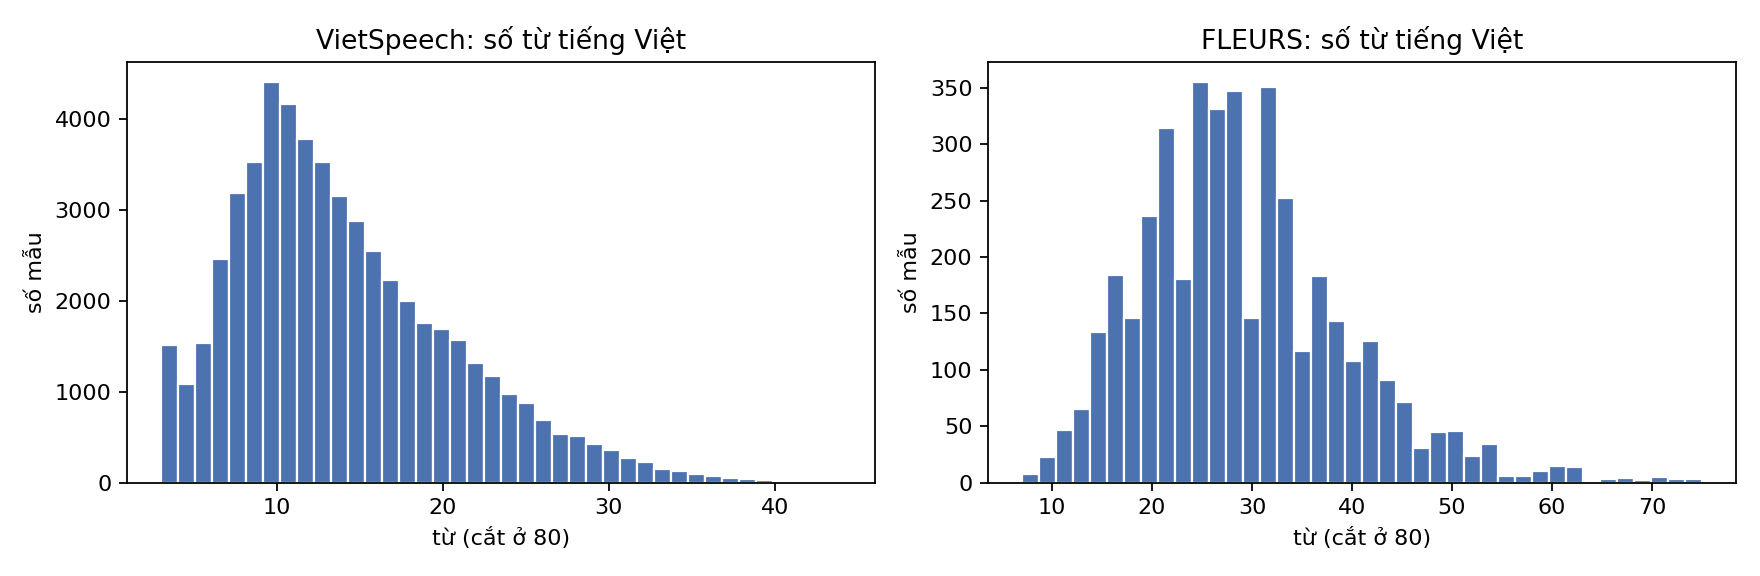
\includegraphics[width=.95\textwidth]{figs/words_hist.png}
\caption{Phân bố thời lượng (trên) và số từ tiếng Việt (dưới): VietSpeech so với FLEURS. Đường đứt đỏ là giới hạn 30 giây của Whisper.}
\end{figure}
\begin{figure}[H]\centering
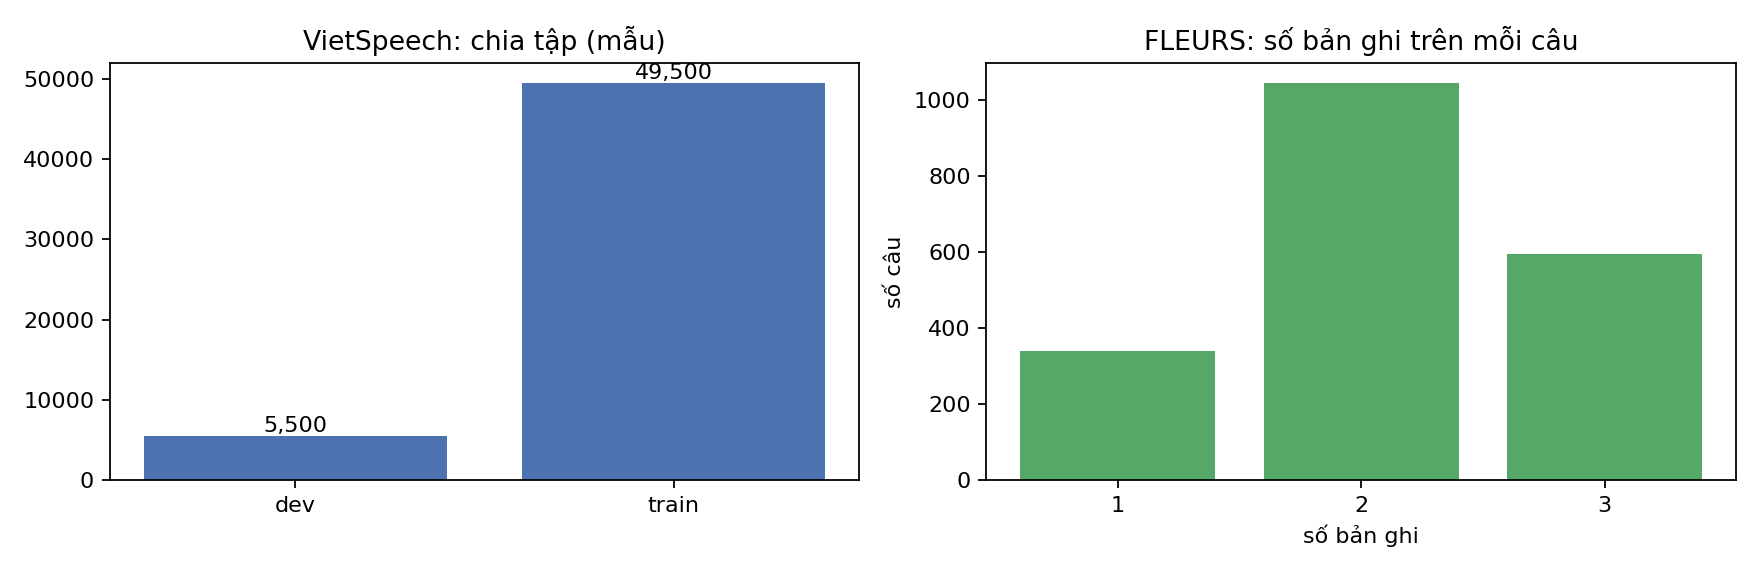
\includegraphics[width=.95\textwidth]{figs/splits_and_records.png}
\caption{Chia tập VietSpeech (trái) và số bản ghi trên mỗi câu của FLEURS (phải).}\label{fig:splits}
\end{figure}
\textbf{Nhận xét định lượng.}
\begin{itemize}[nosep]
\item FLEURS dài hơn VietSpeech khoảng 2,8 lần về thời lượng trung bình (11,3 giây so với 4,0 giây) và 2,0 lần về số từ (29,1 so với 14,3). Toàn bộ VietSpeech ngắn hơn 8 giây, nên mô hình huấn luyện trên VietSpeech chưa từng thấy câu dài hơn 44 từ, trong khi 5\% câu FLEURS dài hơn 48 từ.
\item Số bản ghi trên câu FLEURS: 1\,044 câu có 2 bản ghi, 595 câu có 3 và 339 câu có 1 (Hình~\ref{fig:splits}), nên điểm trung bình theo bản ghi nghiêng về những câu có nhiều giọng đọc; vì vậy khoảng tin cậy lấy mẫu theo câu.
\end{itemize}

\subsection{Đề xuất và kết quả xử lý khác biệt phân bố}
Vì không có mất cân bằng lớp, nhóm không áp dụng class weighting, SMOTE hay focal loss. Các biện pháp xử lý khoảng cách phân bố và độ lệch dữ liệu thực sự được áp dụng:
\begin{itemize}[nosep]
\item \textbf{Fine-tune trên giả thuyết ASR} thay vì transcript sạch, để đầu vào huấn luyện giống đầu vào lúc chạy thật (có lỗi ASR).
\item \textbf{Sửa lỗi nhãn} \texttt{n't} (7,4\% câu).
\item \textbf{Lấy tập con lồng nhau} 25\%, 50\%, 100\% của tập train (12\,375 / 24\,750 / 49\,500 mẫu) để đo ảnh hưởng của lượng dữ liệu.
\item \textbf{Cắt 30 giây và tách riêng} 13 bản ghi dài của FLEURS khỏi điểm chính.
\end{itemize}
Nhóm \emph{không} áp dụng cân bằng lại độ dài (cắt/ghép audio huấn luyện cho dài hơn) hay tăng cường dữ liệu; đây là hướng có thể thử để thu hẹp khoảng cách miền dữ liệu (mục~\ref{sec:v3}). Phân bố trước và sau xử lý được thể hiện ở Hình~\ref{fig:flow} (quy trình) và Bảng~\ref{tab:splits} (55\,000 mẫu chọn từ 100\,000, chia 49\,500/5\,500).

%================ CHƯƠNG II ================
\section{Thực nghiệm hai mô hình Baseline}
\subsection{Môi trường thực nghiệm}
\begin{table}[H]\centering\small
\begin{tabular}{p{5.2cm}p{7.6cm}}\toprule
Thành phần & Giá trị\\\midrule
Phần cứng & GPU NVIDIA Tesla T4 (Google Colab), suy luận fp16\\
Framework & PyTorch, Hugging Face Transformers 5.x\\
Seed & 42 (lấy mẫu dữ liệu, huấn luyện, bootstrap)\\
Beam: ASR / dịch OPUS-MT / Seamless & 3 / 4 / 4\\
Batch suy luận: ASR / OPUS-MT / Seamless & 24 / 64 / 8\\
Giới hạn audio & 30 giây đầu của mỗi bản ghi (cả ba hệ thống)\\
Learning rate, optimizer, epochs & không áp dụng cho A và C (zero-shot, không huấn luyện); thông số của B ở mục~\ref{sec:v1}\\
\bottomrule\end{tabular}
\caption{Cấu hình thực nghiệm.}
\end{table}
Hai baseline là A và C. Cả hai dùng nguyên mô hình công bố, nên không có siêu tham số huấn luyện cần đồng nhất; nhóm đồng nhất dữ liệu đánh giá, phép chuẩn hóa, giới hạn 30 giây, seed và phần cứng.

\subsection{So sánh kết quả công bố và thực nghiệm}
\begin{table}[H]\centering\small
\begin{tabularx}{\textwidth}{>{\raggedright\arraybackslash}p{2.6cm}>{\raggedright\arraybackslash}p{2.4cm}>{\raggedright\arraybackslash}p{2.2cm}Y}\toprule
Mô hình & Nguồn & Chỉ số & Tập đánh giá\\\midrule
PhoWhisper-small & Paper~\cite{phowhisper} & WER 11,08 / 6,33 / 15,93 / 32,96 & CMV-Vi / VIVOS / VLSP2020 Task-1 / Task-2\\
PhoWhisper-small & Nhóm & WER \textbf{11,36} \ci{10,74}{11,99}; CER 7,62 & FLEURS vi (4\,199 bản ghi $\le$ 30 s)\\\midrule
OPUS-MT vi--en & Model card~\cite{opusmt} & BLEU 42,8; chrF 0,608 & Tatoeba-test.vie.eng (câu ngắn)\\
OPUS-MT vi--en (đầu vào ASR) & Nhóm (A) & BLEU \textbf{16,33} \ci{15,74}{16,96}; chrF++ 42,63 & FLEURS vi$\rightarrow$en\\
OPUS-MT vi--en (đầu vào transcript chuẩn) & Nhóm & BLEU 25,91 \ci{25,08}{26,63}; chrF++ 51,30 & FLEURS vi$\rightarrow$en\\\midrule
SeamlessM4T-v2 Large & Paper~\cite{seamless} & BLEU 26,6 (trung bình 81 ngôn ngữ X$\rightarrow$eng); Whisper-Large-v2 + NLLB-3.3B: 22,7 & FLEURS S2TT\\
SeamlessM4T-v2 Large (C) & Nhóm & BLEU \textbf{27,75} \ci{27,04}{28,48}; chrF++ 52,69 & FLEURS vi$\rightarrow$en\\
\bottomrule\end{tabularx}
\caption{Kết quả công bố so với thực nghiệm của nhóm. \textbf{Không có hàng nào cùng tập đánh giá}; xem phân tích ở mục~\ref{sec:gap}. Các số của paper được lấy trực tiếp từ bài báo và model card (ngày truy cập: 25/10/2026).}
\end{table}

\subsection{Phân tích chênh lệch (Gap Analysis)}\label{sec:gap}
\begin{itemize}[nosep]
\item \textbf{PhoWhisper-small.} WER 11,36\% của nhóm gần với 11,08\% (CMV-Vi) nhưng đó là hai tập khác nhau, nên đây \emph{không} phải tái dựng. Paper không công bố kết quả trên FLEURS. Điểm của nhóm bị đẩy lên do không chuẩn hóa số: ASR viết ``hai ngàn không trăm mười lăm'' còn tham chiếu viết ``2015''. Trên các câu có chữ số trong tham chiếu (907 câu, 21,6\%), WER là 27,19\%; trên các câu còn lại (3\,292 câu) WER là 6,81\%, sát mức 6,33\% của VIVOS trong paper (hai tập khác nhau, chỉ so để tham khảo). Chỉ 21 trong 4\,199 đầu ra ASR có chữ số.
\item \textbf{OPUS-MT.} 42,8 BLEU của model card đo trên Tatoeba, gồm các câu ngắn; FLEURS gồm câu dài kiểu văn bản (trung bình 29 từ). Ngay khi đầu vào là transcript chuẩn (không có lỗi ASR) điểm chỉ còn 25,91, nên phần lớn chênh lệch là \emph{khoảng cách miền dữ liệu} (loại câu, độ dài). Thêm lỗi ASR hạ tiếp 9,6 BLEU (còn 16,33); phần này lẫn cả lỗi nhận dạng lẫn khác biệt định dạng (thiếu dấu câu, số bằng chữ), nên không quy hoàn toàn cho lỗi nhận dạng (mục~\ref{sec:gold}).
\item \textbf{SeamlessM4T-v2.} 27,75 BLEU cho vi$\rightarrow$en gần mức trung bình công bố (26,6) nhưng số công bố là trung bình 81 ngôn ngữ; nhóm chưa tìm được số riêng cho tiếng Việt (bảng theo từng ngôn ngữ nằm ở phụ lục bài báo, nhóm chưa tra). Bài báo không nêu rõ FLEURS có nằm trong dữ liệu huấn luyện hay không, nên không loại trừ khả năng FLEURS đã được thấy khi huấn luyện, có thể làm điểm cao hơn thực tế.
\item \textbf{Kỹ thuật tiền xử lý.} Nhóm chuẩn hóa văn bản chỉ khi tính WER (bỏ dấu câu, chữ thường); BLEU/chrF++ tính trên văn bản thô, phân biệt hoa thường, nên thiên về hệ thống C (đầu ra có chữ hoa và dấu câu).
\end{itemize}

%================ CHƯƠNG III ================
\section{Phát triển và đánh giá Proposed Method}
\subsection{Proposed Method V1 (hệ thống B)}\label{sec:v1}
\textbf{Cài đặt.} Fine-tune toàn bộ OPUS-MT vi--en (72,2 triệu tham số) bằng \texttt{Seq2SeqTrainer}: batch 64, learning rate $2\times10^{-5}$, weight decay 0,01, warmup 5\% tổng số bước tối đa (1\,161 bước với 49\,500 mẫu), optimizer mặc định của Trainer (AdamW), tối đa 30 epoch với early stopping theo dev loss (patience 5), fp16, độ dài tối đa 128 token, seed 42. Dữ liệu: 49\,500 cặp train (giả thuyết ASR, nhãn Anh đã sửa \texttt{n't}), dev 5\,500 cặp luôn dùng nguồn ASR.

\begin{table}[H]\centering\small
\begin{tabular}{lrrrrr}\toprule
Lần chạy & Nguồn đầu vào & Mẫu train & Epoch chạy / tốt nhất & Dev loss & Thời gian (phút)\\\midrule
B\_100 & giả thuyết ASR & 49\,500 & 11 / 6 & 1,4645 & 23,8\\
clean\_100 & transcript sạch & 49\,500 & 9 / 4 & 1,5999 & 19,7\\
B\_50 & giả thuyết ASR & 24\,750 & 10 / 5 & 1,5466 & 12,5\\
B\_25 & giả thuyết ASR & 12\,375 & 9 / 4 & 1,6063 & 6,2\\\bottomrule
\end{tabular}
\caption{Bốn lần fine-tune độc lập từ mô hình gốc. Tổng 62,1 phút. Dev loss là loss teacher-forced trên dev VietSpeech (nguồn ASR), \emph{không} phải chất lượng dịch trên FLEURS.}
\end{table}

\begin{table}[H]\centering\small
\begin{tabular}{lcccc}\toprule
Hệ thống & BLEU (KTC 95\%) & chrF++ & $\Delta$BLEU so với A & $\Delta$chrF++\\\midrule
A (baseline 1) & 16,33 \ci{15,74}{16,96} & 42,63 & -- & --\\
B (V1) & 17,24 \ci{16,64}{17,88} & 44,34 & +0,91 \ci{0,50}{1,35} & +1,71\\
C (baseline 2) & 27,75 \ci{27,04}{28,48} & 52,69 & +11,42 \ci{10,74}{12,14} & +10,06\\\bottomrule
\end{tabular}
\caption{Kết quả chính, 4\,199 bản ghi $\le$ 30 giây (1\,974 câu). Trên toàn bộ 4\,212 bản ghi: A 16,29; B 17,19; C 27,69. Trên riêng tập test (850 bản ghi): A 15,47 \ci{14,15}{16,84}; B 16,34 \ci{14,90}{17,91} ($\Delta$ +0,87 \ci{0,01}{1,88}); C 25,60 \ci{24,05}{27,26} ($\Delta$ +10,13 \ci{8,58}{11,69}).}
\end{table}
\begin{figure}[H]\centering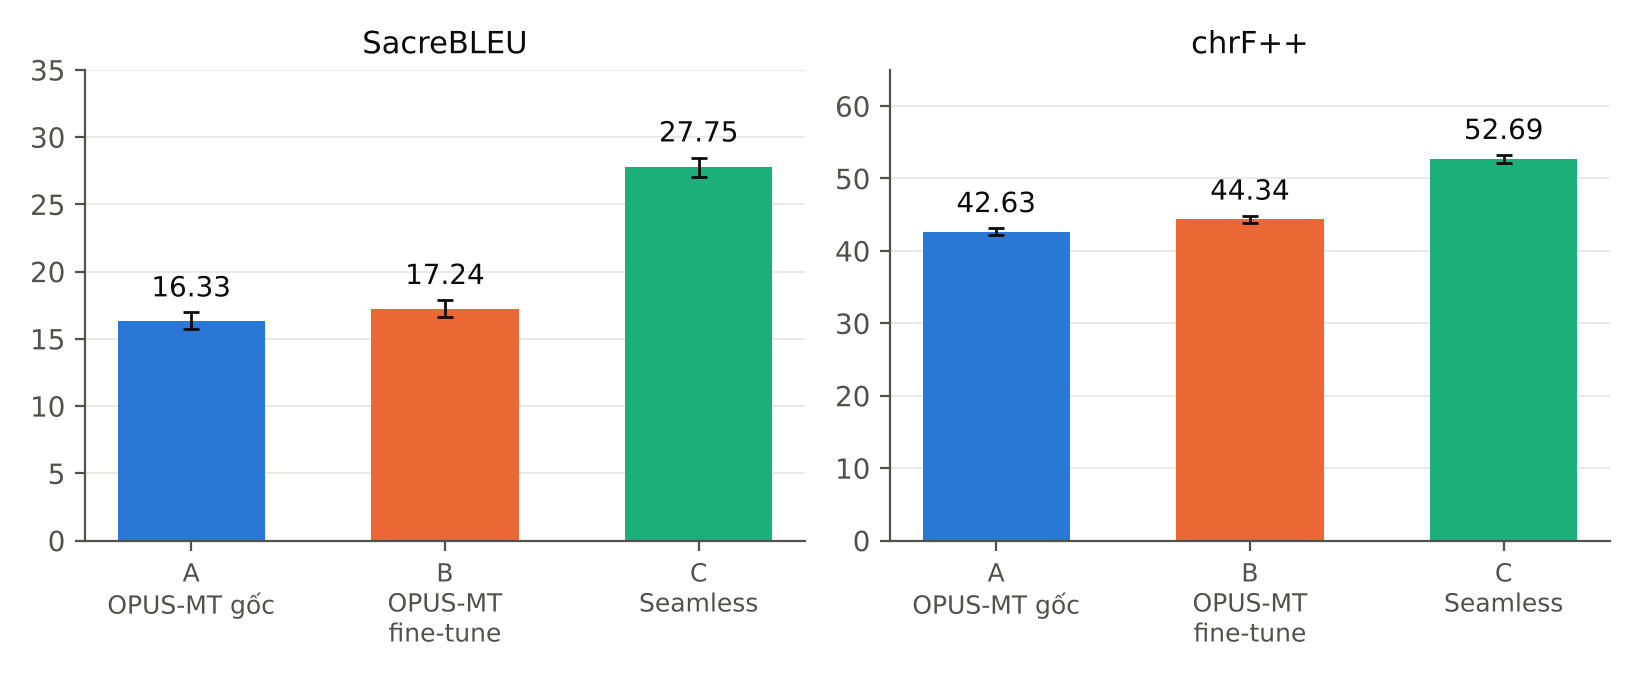
\includegraphics[width=.9\textwidth]{figs/fig_systems.png}
\caption{Điểm A, B, C trên FLEURS (thanh sai số là khoảng tin cậy 95\%).}\end{figure}

\textbf{ASR.} PhoWhisper-small: WER 11,36\% \ci{10,74}{11,99}, CER 7,62\% (4\,199 bản ghi $\le$ 30 s). Theo tập: test 12,16\% \ci{10,84}{13,51}; validation 10,76\% \ci{8,80}{13,06}; train 11,20\% \ci{10,40}{11,98}.

\textbf{Tín hiệu cải thiện.} B vượt A một chút (+0,91 BLEU, khoảng tin cậy không chứa 0 khi gộp; trên riêng tập test cận dưới chỉ 0,01), còn C vượt xa cả hai (+10 đến +11 BLEU). Tín hiệu cải thiện của V1 là \emph{nhỏ nhưng có thật} so với A, và nhỏ so với khoảng cách tới C.

\textbf{Đường cong loss.} Hình~\ref{fig:loss} cho train loss và dev loss theo epoch của bốn lần chạy. Train loss giảm đều (B\_100: từ 1,856 xuống 0,767 sau 11 epoch), trong khi dev loss đạt cực tiểu ở epoch 4--6 (B\_100: 1,4645 ở epoch 6) rồi tăng nhẹ (1,509 ở epoch 11); mô hình bắt đầu quá khớp sau epoch tốt nhất, và early stopping (patience 5) chọn đúng mô hình tại epoch đó. Train loss của clean\_100 thấp hơn ngay từ epoch 1 (1,547 so với 1,856) vì đầu vào sạch dễ hơn đầu vào có lỗi ASR, còn dev loss của nó cao hơn do dev luôn dùng nguồn ASR. Đề yêu cầu confusion matrix và Grad-CAM; hai biểu đồ này không áp dụng cho bài toán sinh văn bản. Nhóm không theo dõi BLEU từng epoch, nên không có đường cong metric dịch.
\begin{figure}[H]\centering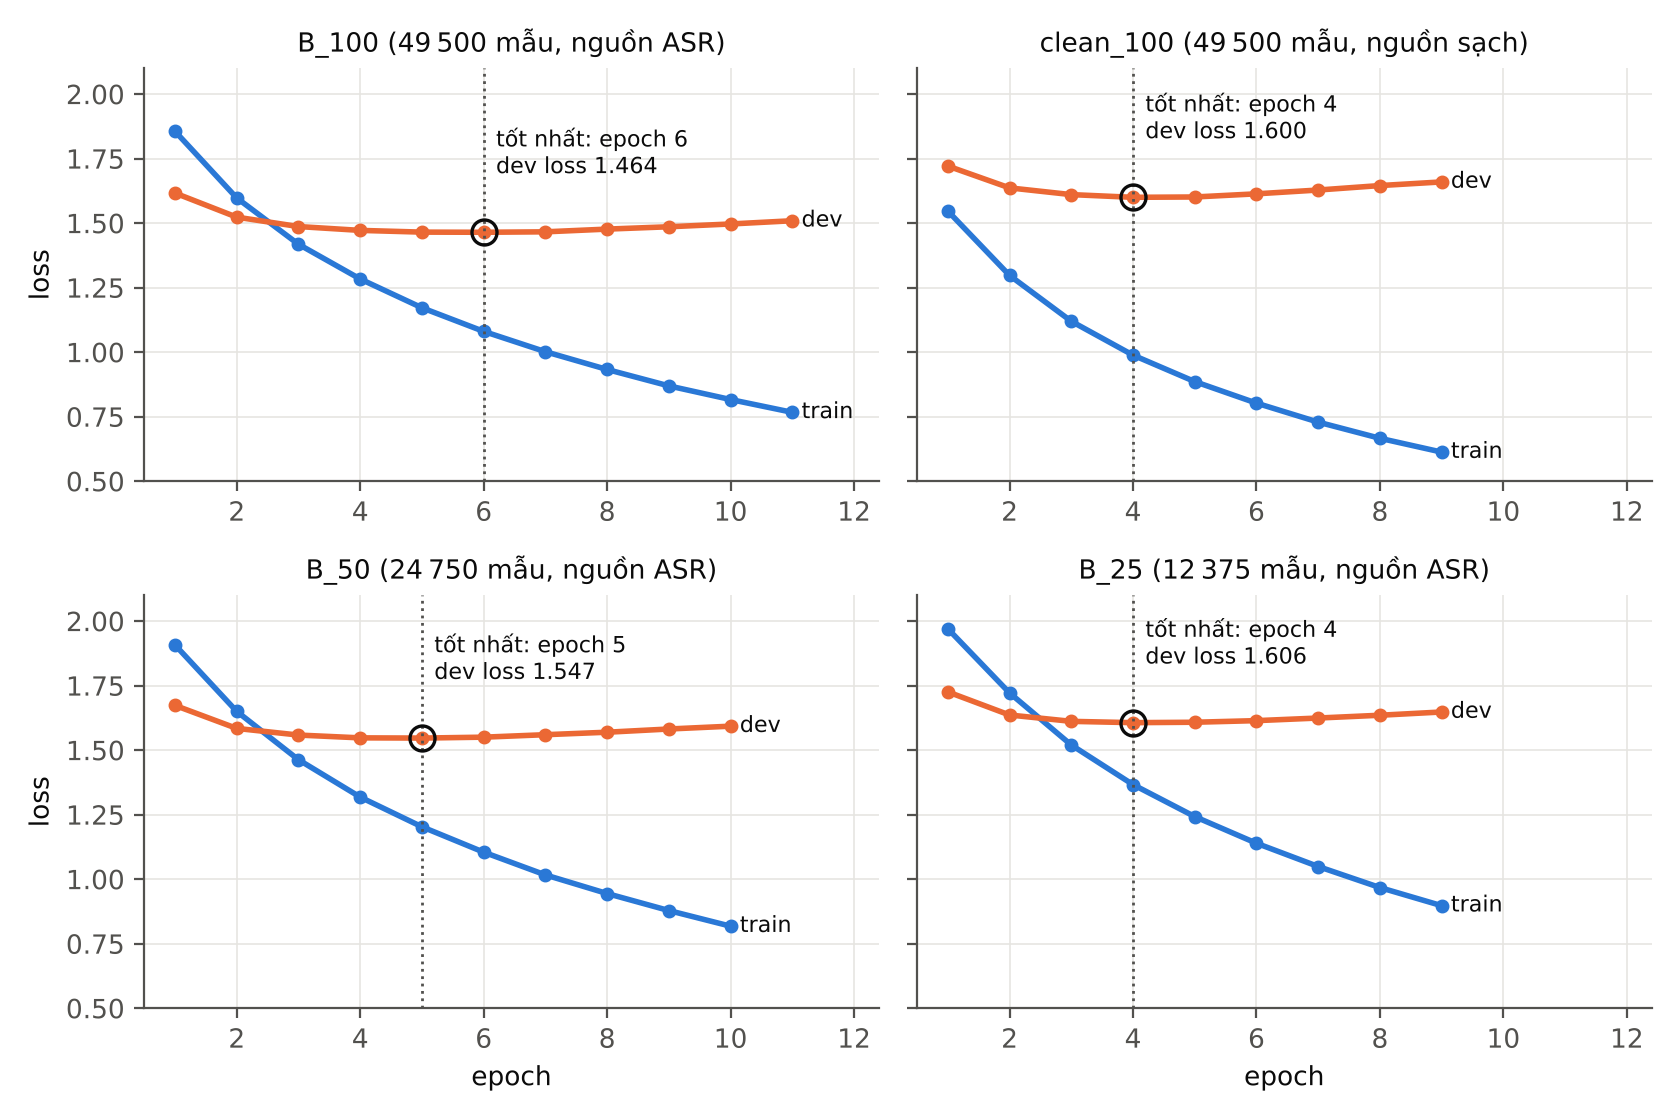
\includegraphics[width=.95\textwidth]{figs/fig_loss.png}
\caption{Train loss (xanh) và dev loss (cam) theo epoch; vòng tròn đánh dấu epoch có dev loss thấp nhất. Dev loss tính trên dev VietSpeech (nguồn ASR).}\label{fig:loss}\end{figure}

\subsubsection{Ablation: nguồn huấn luyện và lượng dữ liệu}
\begin{table}[H]\centering\small
\begin{tabular}{lcccc}\toprule
Hệ thống & BLEU (KTC 95\%) & chrF++ & $\Delta$BLEU so với B\\\midrule
B\_25 (12\,375 mẫu, ASR) & 16,40 \ci{15,77}{17,01} & 43,73 & $-$0,84 \ci{$-$1,17}{$-$0,50}\\
B\_50 (24\,750 mẫu, ASR) & 16,86 \ci{16,24}{17,48} & 44,19 & $-$0,38 \ci{$-$0,69}{$-$0,10}\\
B\_100 (49\,500 mẫu, ASR) & 17,24 \ci{16,64}{17,88} & 44,34 & --\\
clean\_100 (49\,500 mẫu, transcript sạch) & 17,38 \ci{16,77}{18,01} & 44,62 & +0,14 \ci{$-$0,14}{0,40}\\\bottomrule
\end{tabular}
\caption{Ablation (4\,199 bản ghi $\le$ 30 s). Mỗi dòng là một lần fine-tune độc lập từ mô hình gốc, một seed.}
\end{table}
\begin{figure}[H]\centering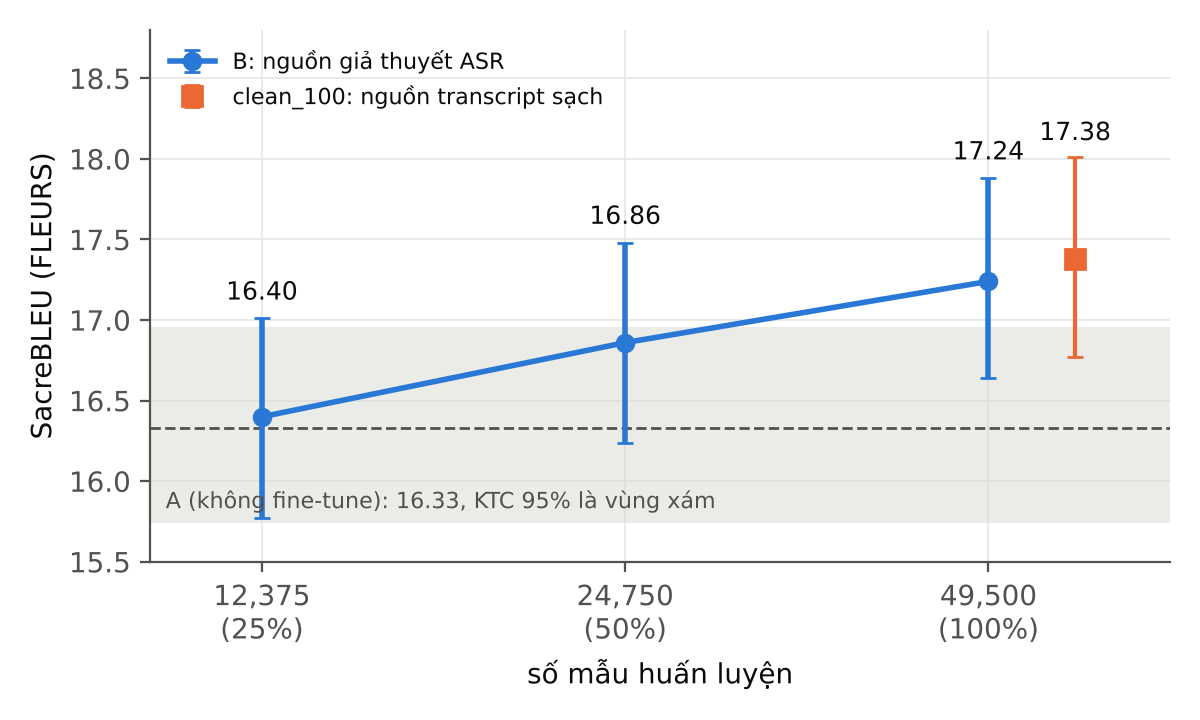
\includegraphics[width=.75\textwidth]{figs/fig_ablation.png}
\caption{Điểm BLEU theo lượng dữ liệu huấn luyện. Vùng xám là khoảng tin cậy 95\% của A.}\end{figure}
\begin{itemize}[nosep]
\item \textbf{Lượng dữ liệu:} nhiều dữ liệu hơn thì điểm cao hơn (16,40 $\rightarrow$ 16,86 $\rightarrow$ 17,24), các chênh lệch khoảng tin cậy không chứa 0; chưa thấy dấu hiệu bão hòa, nên tăng dữ liệu có thể còn cải thiện.
\item \textbf{Nguồn huấn luyện:} \emph{không} có bằng chứng rằng huấn luyện trên giả thuyết ASR tốt hơn huấn luyện trên transcript sạch (+0,14, khoảng tin cậy chứa 0). Giả thuyết ban đầu của nhóm chưa được ủng hộ.
\end{itemize}

\subsection{Phân tích lỗi (Failure Cases) của V1}
Phân tích trên 4\,199 bản ghi $\le$ 30 giây, từ \texttt{fleurs\_all\_outputs.csv}.
\subsubsection{Lỗi lan truyền từ ASR}\label{sec:gold}
Chia câu theo WER của ASR: điểm chrF++ của A giảm từ 46,9 (WER bằng 0, 1\,220 câu) xuống 31,3 (WER trên 40\%, 271 câu); B giảm từ 49,0 xuống 32,5; C gần như phẳng (52,8 xuống 51,4) vì C không đi qua ASR văn bản. Ngay cả khi ASR đúng hoàn toàn, A vẫn thấp hơn C khoảng 6 điểm chrF++.
\begin{figure}[H]\centering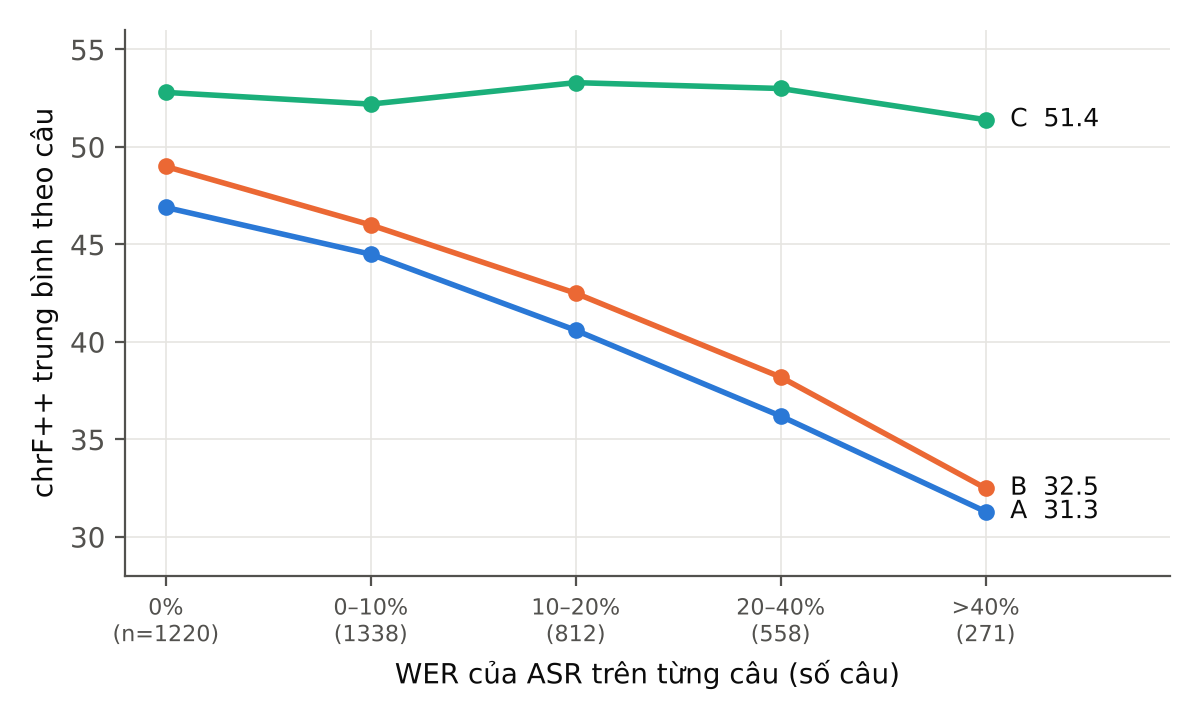
\includegraphics[width=.72\textwidth]{figs/fig_wer_bucket.png}
\caption{chrF++ trung bình theo câu, chia theo WER của ASR trên câu đó.}\end{figure}
Thử dịch từ transcript chuẩn (đầu vào ``gold'') thay vì giả thuyết ASR cho điểm cao hơn rõ rệt (Hình~\ref{fig:gold}), nhưng khoảng chênh \emph{lẫn hai nguyên nhân}: lỗi nhận dạng và khác biệt định dạng (giả thuyết ASR thiếu dấu câu, đọc số thành chữ, chữ thường). Ngoài ra B\_100 với đầu vào gold (22,81) thấp hơn A với đầu vào gold (25,91): fine-tune trên giả thuyết ASR làm giảm chất lượng trên đầu vào chuẩn. Nhóm nghi nguyên nhân là mô hình quen định dạng ASR, nhưng điều này \emph{chưa được kiểm chứng}.
\begin{figure}[H]\centering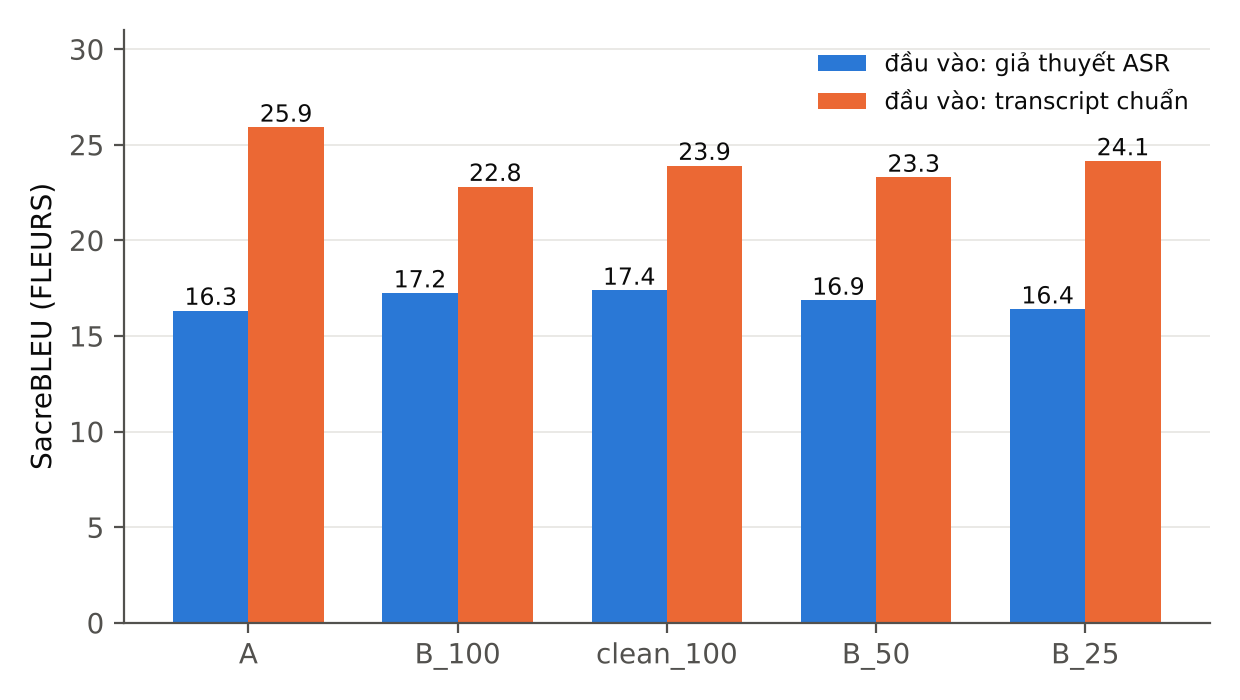
\includegraphics[width=.7\textwidth]{figs/fig_gold.png}
\caption{BLEU khi đầu vào là giả thuyết ASR (xanh) và transcript chuẩn (cam).}\label{fig:gold}\end{figure}

\subsubsection{Các nhóm lỗi định lượng}
\begin{table}[H]\centering\small
\begin{tabularx}{\textwidth}{>{\raggedright\arraybackslash}p{3.6cm}YYY}\toprule
Nhóm lỗi & A & B & C\\\midrule
Câu có số trong tham chiếu (907 câu): BLEU & 11,84 & 12,06 & 29,47\\
Câu không có số (3\,292 câu): BLEU & 17,54 & 19,06 & 27,23\\
Số tham chiếu xuất hiện trong bản dịch (trên 1\,378) & 115 (8\%) & 17 (1\%) & 933 (68\%)\\
Câu có cụm 3 từ lặp từ 3 lần trở lên & 16 & 31 & 11\\
Số từ dịch / số từ tham chiếu & 1,062 & 1,093 & 0,967\\
Câu dịch còn từ có dấu tiếng Việt & 20 & 56 & 18\\\bottomrule
\end{tabularx}
\caption{Thống kê lỗi trên 4\,199 bản ghi. Chữ số ở đầu ra B và A thưa vì ASR đọc số thành chữ.}
\end{table}
\begin{itemize}[nosep]
\item \textbf{Số (21,6\% câu có số).} ASR đọc số thành chữ nên dịch ra chữ (``ten thousand'') thay vì chữ số (``10,000''). Mức tăng của B so với A tập trung ở câu không có số (+1,5 BLEU) và gần bằng không ở câu có số (+0,2).
\item \textbf{Tên riêng và từ mượn.} ASR phiên âm theo âm tiếng Việt và bước dịch không sửa lại được. C nghe trực tiếp nên thường đúng. Tỉ lệ nhóm lỗi này chưa được đếm (cần gán nhãn thủ công).
\item \textbf{Dịch lặp vòng.} Xem bảng và ví dụ bên dưới; B lặp nhiều nhất (31 câu).
\item \textbf{Khác biệt độ dài:} B dịch dài hơn tham chiếu (1,093) và giữ lại nhiều từ có dấu tiếng Việt hơn A (56 so với 20 câu).
\end{itemize}

\subsubsection{Ví dụ tiêu biểu}
\begin{table}[H]\centering\scriptsize\setlength{\tabcolsep}{3pt}
\begin{tabularx}{\textwidth}{>{\raggedright\arraybackslash}p{1.5cm}YYYY}\toprule
Lỗi & Tham chiếu / ASR & A & B & C\\\midrule
Tên riêng (validation/00089) & \emph{NHK also reported that the Kashiwazaki Kariwa nuclear power plant in Niigata prefecture was operating normally.} ASR: ``nhân hàng hát ca cũng thông tin ... ca si qua gia ki ca ri qua ... ni ga ta'' & The line of singing also informs us that the nuclear cassia plant passed through the nitrogen district & -- & The NHK also informed that the Kashiwazaki-Kariwa nuclear plant in Niigata Prefecture was operating normally.\\\midrule
Ký hiệu (train/01252) & \emph{Suspected cases of H5N1 in Croatia and Denmark remain unconfirmed.} ASR: ``hát năm nờ một'' & No, no, no, no, no, no, no, no, ... (lặp) & The suspects sing in the first year in Croatia and Denmark are still not confirmed. & The suspected H5N1 cases in Croatia and Denmark have yet to be confirmed.\\\midrule
Lặp vòng ở B (train/01539) & \emph{A contagious disease is a disease which is easily transmitted by being in the vicinity of an infected person.} & The infectious disease is an easily transmitted disease in the neighborhood of the infected. & It's contagious, it's contagious, it's contagious, it's close to the sick. & An infectious disease is a disease that is easily transmitted when it is in the vicinity of an infected person.\\\midrule
Tên và số (test/00622) & \emph{Goats seem to have been first domesticated roughly 10,000 years ago in the Zagros Mountains of Iran.} ASR: ``... mười ngàn năm ... dưới núi jaguar thuộc iraq'' & ... about ten thousand years ago at the foot of Mount jaguar of iq. & ... ten thousand years ago in the mountains of Jurain in Iraq. & ... about ten thousand years ago in the Zagros Mountains of Iran.\\\midrule
Lặp vòng ở C (train/01852) & ASR lặp nguyên một đoạn (WER 1,08) & ... deers at the lower levels are the ones of the cat-sized family ... & ... catcats ... and South Vietnam at lower levels ... & At the lower levels are cats, the size of a cat, the size of a cat, the size of a cat, ...\\
\bottomrule\end{tabularx}
\caption{Các trường hợp lỗi tiêu biểu (rút gọn bằng dấu ba chấm). Mã trong ngoặc là mã bản ghi FLEURS.}
\end{table}

\subsection{Phiên bản V2: chặn lặp khi giải mã}
\textbf{Lý do (từ phân tích lỗi).} Một số câu dịch bị lặp vòng (16 câu ở A, 31 ở B). \textbf{Thay đổi duy nhất:} thêm \texttt{no\_repeat\_ngram\_size=3} khi giải mã bước dịch; ASR, mô hình và các thiết lập khác giữ nguyên. Dùng lại đầu ra ASR đã lưu; dịch lại 300 câu đầu không bật chặn lặp thì giống V1 ở 300/300 câu (B) và 296/300 câu (A).
\begin{table}[H]\centering\small
\begin{tabular}{lcccc}\toprule
Hệ thống & BLEU (KTC 95\%) & chrF++ & $\Delta$BLEU so với V1 & Câu lặp\\\midrule
V1 A & 16,33 \ci{15,74}{16,96} & 42,63 & -- & 16\\
V2 A & 16,42 \ci{15,81}{17,03} & 42,67 & +0,10 \ci{0,01}{0,20} & 0\\
V1 B & 17,24 \ci{16,64}{17,88} & 44,34 & -- & 31\\
V2 B & 17,38 \ci{16,77}{17,98} & 44,40 & +0,14 \ci{0,04}{0,25} & 1\\\bottomrule
\end{tabular}
\caption{V1 và V2 (4\,199 bản ghi $\le$ 30 s). Trên riêng tập test: V2 B +0,44 \ci{0,14}{0,81} (16,34 $\rightarrow$ 16,77).}
\end{table}
V2 loại gần hết lỗi lặp nhưng điểm tăng rất nhỏ. Tác dụng phụ: \texttt{no\_repeat\_ngram\_size=3} cấm mọi cụm ba từ lặp, kể cả lặp hợp lệ, nên đổi 373 câu của B và 354 câu của A trong khi chỉ khoảng 30 câu bị lặp; một câu có năm tháng bị dịch tệ hơn. V2 được nghĩ ra sau khi đọc đầu ra trên FLEURS (kể cả tập test) nên có yếu tố chọn lọc trên dữ liệu đánh giá; giá trị 3 chưa được dò.

\subsection{Đề xuất V3 (chưa chạy)}\label{sec:v3}
\begin{itemize}[nosep]
\item \textbf{Chuẩn hóa số trước khi dịch:} đổi số bằng chữ trong đầu ra ASR về chữ số. Lý do: 21,6\% câu có số, WER 27\% so với 7\% ở câu không có số, và B chỉ giữ 1\% số của tham chiếu.
\item \textbf{Huấn luyện trộn} giả thuyết ASR và transcript sạch; lý do: B\_100 kém hơn A trên đầu vào chuẩn và không hơn clean\_100.
\item \textbf{Thu hẹp khoảng cách độ dài:} ghép các mẫu ngắn của VietSpeech thành câu dài hơn khi huấn luyện, vì VietSpeech chỉ có mẫu $\le$ 8 giây.
\end{itemize}

\subsection{Bảng theo dõi tiến trình các phiên bản}
\begin{table}[H]\centering\small
\begin{tabularx}{\textwidth}{>{\raggedright\arraybackslash}p{1.4cm}YYcY}\toprule
Phiên bản & Thay đổi so với bản trước & Lý do (từ phân tích lỗi) & BLEU & Nhận xét\\\midrule
A (baseline) & PhoWhisper + OPUS-MT gốc & -- & 16,33 & Mốc so sánh\\
C (baseline) & Seamless S2TT zero-shot & -- & 27,75 & Cao nhất; tham chiếu tốt nhất\\
V1 (B) & Fine-tune OPUS-MT trên giả thuyết ASR (49\,500 mẫu) & Giảm lỗi lan truyền từ ASR & 17,24 & +0,91 so với A; không hơn transcript sạch\\
V2 & + \texttt{no\_repeat\_ngram\_size=3} & Dịch lặp vòng (31 câu ở B) & 17,38 & +0,14 so với V1; loại gần hết câu lặp\\
V3 (đề xuất) & Chuẩn hóa số; huấn luyện trộn & Số và định dạng & -- & Chưa thử\\\bottomrule
\end{tabularx}
\caption{Tiến trình các phiên bản (điểm trên 4\,199 bản ghi $\le$ 30 s).}
\end{table}

\subsection{Đánh giá tính khả thi xây dựng sản phẩm}
\begin{table}[H]\centering\small
\begin{tabular}{lrrrr}\toprule
Thành phần & Tham số (M) & Thời gian (s) & VRAM (GB) & File\\\midrule
PhoWhisper-small (ASR) & 241,7 & 2\,200 & 5,02 & 922 MB\\
OPUS-MT gốc / fine-tune (dịch) & 72,2 & 56 -- 66 & 0,96 -- 1,15 & 274 MB\\
\textbf{A hoặc B (ASR + dịch)} & \textbf{314} & \textbf{$\approx$ 2\,260} & \textbf{5,02} & \textbf{$\approx$ 1,2 GB}\\
\textbf{C: Seamless-v2 (phần S2TT)} & \textbf{1\,501,8} & \textbf{2\,220} & \textbf{5,45} & chưa đo\\\bottomrule
\end{tabular}
\caption{Hiệu năng trên 13,26 giờ audio (4\,212 bản ghi, đã cắt 30 s), Tesla T4, fp16, chạy theo batch. RTF khoảng 0,05 cho cả ba hệ thống (A và B: 0,047; C: 0,047 trước chỉnh). Thời gian của nhóm đầu đã tính cả lúc nạp mô hình; sau khi chỉnh (ước lượng) RTF của C khoảng 0,043 và của ASR khoảng 0,046.}
\end{table}
\textbf{Độ chính xác.} Cao nhất ở C (27,75 BLEU); A và B quanh 16--17. \textbf{Tốc độ.} Cả ba có RTF khoảng 0,04--0,05 khi chạy theo batch trên T4, tức nhanh hơn thời gian thực khoảng 20 lần; đây là \emph{thông lượng}, độ trễ từng câu và hiệu năng một luồng chưa đo. \textbf{Kích thước.} A/B tổng khoảng 314 triệu tham số (1,2 GB); phần Seamless nhóm nạp có 1,50 tỉ tham số (bài báo ghi 2,3 tỉ cho cả mô hình~\cite{seamless}).

\textbf{Kết luận.} Về kỹ thuật, pipeline \emph{có khả thi} để đóng gói thành bản demo chạy trên một GPU cỡ T4: cả ba hệ thống có thông lượng cao hơn nhiều so với thời gian thực và VRAM đỉnh dưới 6 GB. Về chất lượng, hệ thống tự phát triển (B, V2) chỉ cải thiện nhỏ so với baseline A và còn cách C nhiều, nên nếu sản phẩm cần chất lượng dịch cao nhất thì C là lựa chọn tốt nhất theo dữ liệu hiện có; nếu cần mô hình nhỏ hơn thì A/B/V2. Môi trường triển khai phù hợp là một ứng dụng gọi mô hình chạy trên server có GPU; trước khi đóng gói cần đo thêm độ trễ từng câu và hiệu năng với giọng nói tự nhiên, những việc chưa thực hiện.

%================ HẠN CHẾ ================
\section{Hạn chế và lưu ý}\label{sec:limit}
\begin{itemize}[nosep]
\item Mỗi lần fine-tune chỉ một seed; chưa đo độ biến thiên giữa các seed.
\item Khả năng FLEURS đã nằm trong dữ liệu huấn luyện của Seamless chưa được kiểm chứng.
\item Khoảng chênh giữa đầu vào ASR và đầu vào chuẩn lẫn lỗi nhận dạng với khác biệt định dạng (mục~\ref{sec:gold}).
\item WER không chuẩn hóa số nên bị đẩy lên; BLEU phân biệt hoa thường và tính trên văn bản thô.
\item Nhãn tiếng Anh của VietSpeech là nhãn giả từ VinAI Translate v2, chưa kiểm tra chất lượng bằng người; chưa kiểm tra trùng nội dung trong VietSpeech.
\item V2 được chọn sau khi xem đầu ra FLEURS (kể cả tập test); điểm V2 có yếu tố chọn lọc trên dữ liệu đánh giá.
\item Thời gian của nhóm đầu tiên mỗi giai đoạn gồm cả lúc nạp mô hình; số RTF sau chỉnh chỉ là ước lượng. Suy luận fp16 theo batch có thể lệch rất nhỏ giữa các lần chạy (A: 296/300 câu giống hệt khi dịch lại).
\item Chưa có đánh giá bởi người; chưa đo độ trễ từng câu và hiệu năng với giọng nói tự nhiên của cuộc họp.
\end{itemize}

%================ PHỤ LỤC ================
\appendix
\section{Tái lập kết quả}
\begin{table}[H]\centering\small
\begin{tabularx}{\textwidth}{>{\raggedright\arraybackslash}p{4.6cm}Y}\toprule
Notebook & Nội dung / đầu ra\\\midrule
\texttt{ASR\_PhoWhisper\_zip\_parts} & ASR VietSpeech (beam 3), \texttt{results/asr\_out/asr\_hyp.csv}\\
\texttt{MT\_opus\_finetune} & Bốn lần fine-tune, \texttt{results/ft\_out/*/best\_model}\\
\texttt{FLEURS\_eval\_ABC} & ASR + dịch A/B + Seamless C + bảng điểm; \texttt{results/fleurs\_out/}\\
\texttt{FLEURS\_V2\_norepeat} & V2 chặn lặp; \texttt{results/fleurs\_out/v2/}\\
\texttt{Stats\_for\_report} & Thống kê dữ liệu, kích thước mô hình; \texttt{results/stats/}\\\bottomrule
\end{tabularx}
\end{table}
Tập con VietSpeech: hoán vị seed 42 của 100\,000 mẫu đầu có transcript hợp lệ, vị trí $[0, 5\,500)$ là dev, $[5\,500, 55\,000)$ là train; các tập 25\%/50\% là tiền tố của train theo vị trí.

\begin{thebibliography}{9}
% Chỉ dẫn nguồn của hai baseline: A (PhoWhisper + OPUS-MT) và C (Seamless).
\bibitem{phowhisper} VinAI Research, ``PhoWhisper: Automatic Speech Recognition for Vietnamese'', arXiv:2406.02555. \url{https://arxiv.org/pdf/2406.02555}
\bibitem{opusmt} Helsinki-NLP, ``opus-mt-vi-en'' (model card). \url{https://huggingface.co/Helsinki-NLP/opus-mt-vi-en}
\bibitem{seamless} Seamless Communication \emph{et al.}, ``Seamless: Multilingual Expressive and Streaming Speech Translation'', arXiv:2312.05187. \url{https://arxiv.org/pdf/2312.05187}
\end{thebibliography}
\end{document}
